\newpage
\chapter{Methodology}
In the following chapter, the component analysis is defined first. This results in the requirements that must be considered in the design when implementing the extension, which is then discussed in the third section. In the final section, the tests, to ensure that the extension matches the expected requirements and it is defect free, are described.

\section{Design Concept}
The original concept of this thesis is to create an additional feature for marta's customer-facing platforms. \emph{Marta}\footnote{\emph{Marta} can be accessed through \url{https://www.marta.de/}} as a business is currently best described as a marketplace between caregivers and families requiring 24-hour care. 24-hour care can be defined as living in a household with the person in need of care for a certain period of time. This means that caregivers are primarily responsible for basic care and household chores. In addition, they support the person in care's relatives in need of assistance in carrying out the activities they wish to do. Marta as a marketplace connecting families with caregivers is competing against more traditional agencies, where it can take several days or even weeks to find a family for a newly signed up caregiver or the other way around.

As a growing start-up that gained a lot of users in the past few months, marta would need to enhance their product, to compete in this expeditiously developing business. One way marta can provide a superior experience for both caregivers and families is to speed up the matching process between both parties. The caregiver and family inquiry forms are designed to record as much information as possible which can be used during the matching phase. The matches are then created by the teams in Berlin and Romania. To make the job more seamless, the technical team in marta introduced a "matching score" by which possible matches are sorted. As a result, a number of caregiver profiles with high matching scores are shown to the family. Filter functionality is provided to speed up the search process. This includes caregiver's earliest starting date, German skills, experience with diseases, etc.

Marta needs to introduce a continually improved, user-friendly filtering functionality to adjust to the needs of their users. An example of a user-friendly filter would be to provide quick filter suggestions which the user can click once and the desired results will be shown, instead of letting users select the same filter manually over and over again. In order to determine which filter suggestions are the most beneficial, frequently used filters need to be identified.

A question arose within this world of thought about how to improve the existing filtering functionality for a better user experience. An early concept was to create quick filters within the application that suggested to users which filters they frequently used. For example, if a family is looking for a caregiver with German speaking capability level 3, the German filter would be activated. Each filter usage will be counted and saved to a relational database. The three most frequently used filters will be displayed as quick filters for all users, and the user will only need to click on those quick filters to activate them. Not only that, the user can also combine those quick filters to narrow the search even further.

The first problem with this idea was that it collected filter usage data from every user and stored it without providing any detailed information about who used the filter and when it was used. Each family's search criteria are unique. Hence the first idea would not be as beneficial to the users. We must also keep in mind that this approach will only benefit those who actively use the platform. The second concern was that if the filter recommendations were tailored to each individual user, the amount of data maintained would rapidly grow to be rather large. It would be a waste of storage space and would not be sustainable, especially if the number of filters and users grows. We would develop quick filters not only on one page, but on several. And each would require the same amount of storage space.

The concept was then expanded upon and a decision was reached. Instead of adding those quick filters directly into the platform, an extension that allows for even more personalized filter suggestions should be developed. The aforementioned issues can be addressed by developing an extension. The information that will be saved varies for each user and is saved in the end user's browser, which means that other users' activity will not impact the filter suggestions. Furthermore, search and filter is a popular website design method. It would benefit not just Marta's platform, but also other e-commerce websites like Lacoste, Nike, Adidas, and others. Moving it to an extension would allow people to choose whether or not to install it. And, because this is a separate capability with a different software architecture than Marta's primary platform, a new repository or codebase is developed to make it easier to distinguish and manage.

\section{Requirements Elicitation and Analysis}
\label{requirements_analysis}
The extension is used to improve the user's experience when navigating through an e-commerce website to search for a wanted product or service. The idea is to integrate the end user's browser with an extension, which will record the host name or domain of the visited website's URL along with the respective parameters. When enough records have been collected, the extension will display a list of parameters for the visited domain. Path parameters and query parameters will be separated from these parameters. The user can then navigate through the path parameters in the same way that they would navigate through a file system. When a path with parameters is reached, the query parameters and the number of times these parameters are called in the URL are displayed. Below the list is an input field and a button; this input field is filled based on and while navigating through the selected parameters. When the "Navigate" button is clicked, a new tab opens with the full-path built URL.

Jakob Nielsen's third usability heuristic for user interface design is user control and freedom. This principle states:

\begin{displayquote}
  Users often choose system functions by mistake and will need a clearly marked "emergency exit" to leave the unwanted state without having to go through an extended dialogue. Support undo and redo \autocite{nielsen1994usability}.
\end{displayquote}

\noindent With this in mind, the user should be able to return after moving forward. A close button should be provided to make it clear to users how to exit the extension. To broaden the definition of "control," users should also have the ability to customize; they should be able to choose which query parameters should be saved and which should not.

These prerequisites and considerations result in the following requirements for the extension, which is to be developed within the scope of this thesis. These requirements are classified into functional and non-functional requirements.

\subsection{Functional Requirements}
A requirement is called functional if its underlying need is functional, i.e., it relates to information processing objects (data, operations, behavior). In other words, functional requirements are statements of services the system should provide, how the system should react to particular inputs and how the system should behave in particular situations \autocite{sommerville2011software}. The following functional requirements are defined for the extension:

\begin{itemize}
  \item FR-01: User can see how many times each query parameters for each host name and path name are used
  \item FR-02: User can see a list of paths and parameters based on their history
  \item FR-03: User can assemble a URL query string by selecting a path or a parameter
  \item FR-04: User can navigate to the URL with the assembled query string
  \item FR-05: The extension saves the host name, pathname and query parameters of the URL
  \item FR-06: The extension stores the URL attributes each time a page is loaded
  \item FR-07: User can define which query parameters should be excluded in the options page
  \item FR-08: User can remove a query parameter count by clicking on remove icon
  \item FR-09: User can clear all the filter from the options page
  \item FR-10: User can reset the configuration from the options page
\end{itemize}

In addition to functional requirements, non-functional requirements are also defined as follows.

\subsection{Non-Functional Requirements}
A requirement is called non-functional if its underlying need is a non-objective property. In other words non-functional requirementes are constraints on the services or functions offered by the system such as timing constraints, constraints on the development process, standards, etc \autocite{sommerville2011software}. It often apply to the system as a whole rather than individual features or services. The following non-functional requirements arise for the extension to be developed:

\begin{itemize}
  \item NFR-01: UI components must be implemented using React.
  \item NFR-02: TypeScript must be used to implement dynamic functions.
  \item NFR-03: Data must be saved on the end-user's Chrome storage.
  \item NFR-04: User's configuration from the options page must be saved on the end-user's Chrome storage.
  \item NFR-05: Both the external components used and the developed component itself must be well documented.
  \item NFR-06: The individual external libraries must be easy to update.
  \item NFR-07: Modularization must be taken into consideration throughout development so that individual modules and/or components can be easily reused, expanded or changed.
\end{itemize}

While functional requirements are perceived as such by the user, non-functional requirements are implementation details that remain largely hidden from the user.

\section{Technologies}
\label{technologies_used}
The following section argues the decision about the choice of implementation browser. This affects how the data can be stored when the extension is implemented, which is discussed in the second section.

\subsection{Choice of Implementation Browser}
The selection of a browser was based on a number of factors. The first was the browser's usage rate. This is significant since anyone who doesn't already have the necessary browser will need to download and install it. Drop-outs due to the installation process or being unfamiliar with a new browser can significantly raise the cost of conducting the survey. The ease of use of the API and simplicity of implementation were additional crucial criteria. The extension programming process should ideally only need a basic understanding of the extension API. The capabilities of the API offered by the browser was another factor considered. The extension needs to:

\begin{enumerate}
  \item Store a big amount of data on the client side
  \item Read URL - so path and query string can be passed to the extension
  \item Modify URL - so frequently used path and query string can be utilized
  \item Open a full-path URL in a new tab
  \item Access opened tabs
\end{enumerate}

After more than 25 years of helping people use and experience the web, \emph{Internet Explorer}\footnote{\emph{Internet Explorer} is a World Wide Web browser that comes bundled with the Microsoft Windows operating system. The browser was deprecated in Windows 10 in favor of Microsoft's new Edge Browser.} is officially retired and out of support as of June 15, 2022. Thus, Internet Explorer was eliminated from the list, leaving Firefox and Chromium-based browsers (such as Google Chrome, Microsoft Edge, Opera, Vivaldi) as the options.

Both the Firefox and Chrome extension APIs provided comparable functionality. To a considerable degree, Firefox's extension technology is compatible with the extension API used by Chromium-based browsers. Most extensions designed for Chromium-based browsers operate in Firefox with very minor modifications. One disadvantage was that Mozilla only support Manifest V2 and not V3. Since announcing Manifest V3 in 2018, Google has launched Manifest V3 in Chrome, started accepting Manifest V3 extensions in the Chrome Web Store, co-announced joining the W3C WebExtensions Community Group (formed in collaboration with Apple, Microsoft and Mozilla), and, most recently, laid out a timeline for Manifest V2 deprecation. New Manifest V2 extensions will no longer be accepted as of January 2022, and Manifest V2 will no longer function as of January 2023 \autocite{alexei2021manifest}. Manifest V3 dictates an ecosystem change that limits Manifest V2 extensions and would likely force Manifest V2 based extensions to conform to Manifest V3 in the near future.

\begin{figure}[H]
  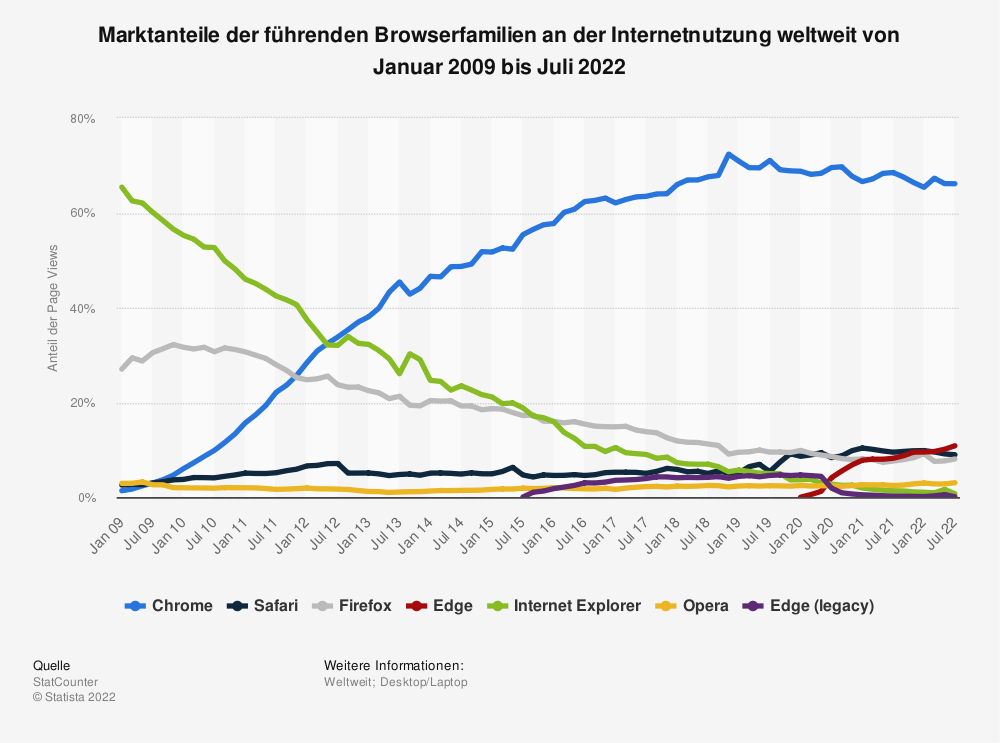
\includegraphics[width=\textwidth]{assets/statistic_id157944_marktanteile-fuehrender-browser-weltweit-bis-juli-2022.png}
  \caption{Market shares of leading browsers worldwide by July 2022}
  \label{fig:browserMarketShareChart}
\end{figure}

Additionally, it was discovered that the Chrome documentation was easy to grasp and was divided up into sections. Chrome also has an overwhelming market share: over two-thirds of all users globally use Chrome as their browser (See \autoref{fig:browserMarketShareChart}). As a result, it was decided to develop a Chrome-based browser extension.

\subsection{Data storage}
Extensions can store data in two places: (1) on the web server or (2) on the web client (the end-user's-computer). Certain data types belong on one, while others perform better on the other. Sensitive and fragile data, for example, should always be stored on the server, whereas static data and user preferences can be stored on the client \autocite{macdonald2013html5}. Currently, most organizations manage various data aspects through various record systems. They have difficulty locating appropriate data stores because they report on each data source separately, resulting in complex data analytics processing. For this project, the types of data that must be stored are specified in \autoref{requirements_analysis}. Since no servers are needed for this project, data is stored and manipulated in the browser --- also known as client-side-storage. Examples of data storage and manipulation scenarios in the browser include:

\begin{itemize}
  \item Preserving the state of a client-side application, such as the current screen, entered data, user preferences, and so on.
  \item Utilities that access local data or files and have strict privacy requirements.
  \item Offline progressive web apps (PWAs)
\end{itemize}

\subsection*{Cookies}
HTTP cookies, or simply cookies, were designed to store session information on the client. As part of any response to an HTTP request, the server was required to send a Set-Cookie HTTP header containing session information, according to the specification. A server response's headers, for example, might look like this:

\begin{lstlisting}[language={}, caption={Cookie server response's headers}]
  HTTP/1.1 200 OK
  Content-type: text/html
  Set-Cookie: name=value
  Other-header: other-header-value
\end{lstlisting}

This HTTP response creates a cookie called "name" with the value "value." When sent, both the name and the value are URL-encoded. Browsers save such session information and send it back to the server via the Cookie HTTP header for each subsequent request, as shown below:

\begin{lstlisting}[language={}, caption={Cookie HTTP header}]
  GET /index.jsl HTTP/1.1
  Cookie: name=value
  Other-header: other-header-value
\end{lstlisting}

This additional data returned to the server can be used to uniquely identify the client from which the request was sent. Although cookies provide a simple and well-supported storage mechanism, they have a number of drawbacks. To begin, each cookie is sent back and forth with each HTTP request (via HTTP headers), adding a significant amount of unnecessary overhead. Second, their storage capacity is far insufficient for modern web applications. Third, the same web application that uses cookies cannot run in multiple web browser tabs at the same time. Finally, the API is somewhat clumsy \autocite{kessin2011programming, macdonald2013html5}.

\subsection*{Web Storage}
The Web Applications 1.0 specification of the Web Hypertext Application Technical Working Group (WHAT-WG) was the first to address web storage. This specification's early development became part of HTML5 before being broken off into its own specification. Its goal is to circumvent some of the constraints imposed by cookies when data is required solely on the client side, without the need to send data back to the server on a constant basis. The Web Storage specification's most recent revision is the second edition. The Web Storage specification's two key goals are to provide a system for storing large amounts of data that survives between sessions and to provide a way to store session data outside of cookies \autocite{frisbie2019professional}.

The Web Storage specification's second edition comprises definitions for two objects: \texttt{localStorage}, the permanent storage mechanism, and \texttt{sessionStorage}, the session-scoped storage mechanism. The \texttt{localStorage} object is kept until it is explicitly erased via JavaScript or until the user clears the browser's cache. Data from \texttt{localStorage} will be retained even after page reloads, closing windows and tabs, and restarting the browser. On the other hand, the \texttt{sessionStorage} object only keeps data for a single session, which means the data is kept until the browser is closed. This is similar to a session cookie, which is deleted when the browser is closed. Data stored on \texttt{sessionStorage} endures through page refreshes and, depending on the browser vendor, may also be available if the browser crashes and is restarted. Both of these browser storage APIs provide two distinct methods for saving data in the browser that can withstand a page reload. Both \texttt{localStorage} and \texttt{sessionStorage} are available as window properties in all major vendor browser releases since 2009.

Web Storage, like other client-side data storage solutions, has limitations. These are browser-specific restrictions. In general, the client-side data size limit is set per origin (protocol, domain, and port), so each origin has a fixed amount of space to store its data. This restriction is enforced by analyzing the origin of the page that is storing the data. Aside from that, Web Storage operates synchronously and will block the main thread. Furthermore, it is inaccessible to web workers or service workers and can only contain strings.

\subsection*{IndexedDB}
The Indexed Database API, abbreviated IndexedDB, is a structured data store in the browser. IndexedDB was created as a replacement for the now-deprecated Web SQL Database API. The goal of IndexedDB was to create an API that allowed for the simple storage and retrieval of JavaScript objects while also allowing for querying and searching. IndexedDB is intended to be almost entirely asynchronous. As a result, the majority of operations are performed as requests that will be executed later and produce either a successful or an error result. To determine the outcome of nearly every IndexedDB operation, you must attach \texttt{onerror} and \texttt{onsuccess} event handlers.

It is an asynchronous, key-value browser-based NoSQL (Not Only SQL) data store. NoSQL is a database approach that is not relational or object oriented. Rather, NoSQL stores data in key/value format. Furthermore, the database can handle a large amount of data and has an API that provides quick access to an unlimited amount of structured data. However, IndexedDB may be considered insecure because security was not a consideration in its design.

IndexedDB has been eliminated from the list for the same reason that Web Storage has been removed. First, IndexedDB databases are tied to the page's origin (protocol, domain, and port), so information cannot be shared across domains. This means that \url{www.wrox.com} and \url{p2p.wrox.com} have their own data stores. Second, IndexedDB is extremely slow, even slower than a database on a low-cost server. Inserting hundreds of documents can take several seconds. Time is important for a quick page load. Even sending data to the backend over the internet can be faster than storing it in an IndexedDB database. Third, a workaround is required for IndexedDB to function alongside the Chrome extension. IndexedDB is a low level API that requires significant setup before use, which can be particularly painful for storing simple data. Unlike most modern promise-based APIs, it is event based. Promise wrappers like \emph{idb}\footnote{\emph{idb} is a tiny library that mostly mirrors the IndexedDB API, but with small improvements that make a big difference to usability. GitHub repository: \url{https://github.com/jakearchibald/idb}} for IndexedDB hide some of the powerful features but more importantly, hide the complex machinery (e.g. transactions, schema versioning) that comes with the IndexedDB library.

\subsection*{Chrome Storage API}
Google Chrome provides an API called \texttt{chrome.storage}. This API has been optimized to meet the specific storage needs of extensions \autocite{chrome2021storage}. It allows you to directly synchronize data and persist data across tabs. Asynchronous storage ensures that scripts are not interrupted. As a result, asynchronous saving outperforms synchronous saving in terms of performance. The asynchronous behavior must be considered during implementation. Web Storage or \texttt{localStorage} has a maximum memory limit of 5 MB and does not support tab-spanning storage because the data is only available in the current context. The cross tab storage and readout is required for the extension's development. It has more or less the same storage capabilities as the \texttt{localStorage} API, with the following important differences:

\begin{itemize}
  \item Using \texttt{storage.sync} user data can be automatically synced.
  \item Without the need for a background page, the extension's content scripts can directly access user data.
  \item Even when using split incognito behavior, a user's extension settings can be saved.
  \item It is faster than the blocking and serial \texttt{localStorage} APIs because it is asynchronous with bulk read and write operations.
  \item Objects can be used to store user data (the \texttt{localStorage} API stores data in strings).
  \item The administrator's enterprise policies for the extension can be read (using \texttt{storage.managed} with a schema).
\end{itemize}

Using \texttt{chrome.storage} can alleviate the aforementioned limitations with other client-side data storage solutions. Chrome Storage API is well-documented, simple, and takes very little time to set up. Data stored in \texttt{chrome.storage} can be accessed not only from tabs and windows of the same origin. The maximum amount of data that can be stored in local storage is 5MB, as measured by the JSON stringification of each value plus the length of each key. However, this value can be ignored if \texttt{unlimitedStorage}\footnote{This permission applies only to Web SQL Database and application cache (see issue \url{https://bugs.chromium.org/p/chromium/issues/detail?id=58985}). Also, it doesn't currently work with wildcard subdomains such as \url{http://*.example.com}.} permission is used. Due to the limitations of HTML5 storage in the context of developing a Chrome Extension, the decision is made to use \texttt{chrome.storage}.
